\documentclass[a4paper,10pt]{article}

% Packages
\usepackage[utf8]{inputenc}
\usepackage[frenchb]{babel}
\usepackage{graphicx}
\usepackage{url}
\usepackage{hyperref}
\usepackage{a4wide}
\usepackage{amsmath}
\usepackage{../p1/clrscode3epg}
\usepackage{color}
%\usepackage{fullpage}
%\renewcommand{\labelenumi}{(\alph{enumi})}

% Style
\parskip=\smallskipamount

% En-têtes
\title{
    \textbf{Structures de données et algorithmes}\\
    {Projet 3\\Mise en page automatique d'une bande dessinée}
}

\author{Pierre \textsc{Geurts} -- Gilles \textsc{Louppe} -- Thomas \textsc{Désir}}
\date{\today}

% Corps
\begin{document}
\maketitle

L'objectif du projet est d'implémenter un algorithme de remise en page
``intelligent'' de bandes dessinées.  Ce projet vous permettra de
mettre en \oe uvre les techniques de résolution de problèmes vues au
cours théorique (essentiellement la programmation dynamique).

Le projet est à réaliser par groupes de {\bf deux} étudiants pour le
{\bf 16 mai 2014} à {\bf 23h59} (du matin) au plus tard. Le projet est
à remettre via une interface web disponible sur
\href{http://www.montefiore.ulg.ac.be/~glouppe/2012-2013/students.info0902.php}{la
  page des TPs}. Utilisez l'identifiant d'un des membres du groupe
pour soumettre votre projet et \textbf{indiquez les noms et matricules
  de chacun des membres sur le rapport et dans chacun des fichiers
  sources}.

Un projet non rendu à temps recevra automatiquement une cote nulle. En
cas de plagiat avéré, l'étudiant se verra affecter une cote nulle à
l'ensemble du projet. Soyez bref mais précis dans votre rapport et
respectez bien la numérotation des sous-questions de l'énoncé.

Les critères de correction sont précisés sur la page web des projets.

\section{Description du programme}

Le programme qu'on vous demande d'implémenter prendra en entrée une
série ordonnée de cases de bande dessinée (c'est-à-dire des images) et
une largeur de page et devra fournir en sortie une nouvelle image de
cette largeur sur laquelle les cases auront été rangées de gauche à
droite et de bas en haut. Ces cases auront également été étirées ou
réduites grâce à une technique particulière, appelée ``Seam carving''
\cite{seamcarving}, de manière à occuper {\bf complètement} (aux bords
près) la largeur de l'image générée. Des exemples de résultats de
l'application de ce programme sont montrés sur la page web des projet.

L'implémentation de cette méthode se fera en deux étapes:
\begin{itemize}
\item \`A partir de la largeur de page fournie et des largeurs des
  différentes cases\footnote{On supposera qu'elles ont toute la même
    hauteur.}, on déterminera le nombre de rangées de la page finale
  et la répartition des différentes cases sur ces rangées. Cette
  répartition sera déterminée à l'aide d'un algorithme généralement
  utilisé pour faire de la justification de texte.
\item \`A partir de la répartition obtenue des cases sur les
  différentes rangées de la planche, on déterminera pour chaque rangée
  si les cases doivent être réduites ou étendues de manière à remplir
  complètement la largeur de la page. Ces transformations seront
  ensuite appliquées aux cases en utilisant l'algorithme de Seam
  Carving et les cases ainsi transformées seront placées (de gauche à
  droite et de haut en bas) sur l'image finale.
\end{itemize}
L'algorithme de répartition des cases et le seam carving font tous
deux appel à la programmation dynamique. Ces deux algorithmes sont
décrits ci-dessous.

\subsection{Algorithme de répartition des cases}

L'algorithme pour déterminer le placement des cases sur l'image finale
de largeur donnée $W$ est similaire à un algorithme de justification
de texte\footnote{\`A la modification près, qu'ici, on permettra aux
  cases de dépasser a priori les limites de la page, dans la mesure où
  on pourra les réduire.}. \`A partir d'un tableau $l[1\twodots n]$
contenant les largeurs, en nombre de pixels, des $n$ cases dans leur
ordre d'apparition sur la planche, il s'agit de déterminer un
placement des cases rangée par rangée. Ce placement sera déterminé
avec pour objectif de minimiser les transformations de largeur des
cases, c'est-à-dire en minimisant pour chaque rangée le nombre de
pixels à remplir (par un élargissement) ou à gagner (par une
réduction) pour satisfaire la contrainte de largeur de page.

De manière plus formelle, afin de définir le coût d'une répartition,
on définira les deux fonctions (ou tableaux) suivantes:
\begin{itemize}
\item $extras(i,j)$ (pour $1\leq i\leq j\leq n$) qui calcule la
  différence entre la largeur de la page $W$ et la somme des largeurs
  des cases $i$ à $j$. $extras(i,j)$ représentera donc l'espace vide
  ou l'excédent par rapport $W$ lorsqu'on place les cases $i$ à $j$
  sur une même rangée.
\item $cost(i,j)$ (pour $1\leq i\leq j\leq n$) attribuant un coût au
  placement des cases $i$ à $j$ sur la même rangée. Plusieurs
  définition de coût sont possible. Dans le cadre du projet, on vous
  propose d'utiliser comme valeur de coût $c(i,j)=(|extras(i,j)|)^3$,
  qui pénalise de manière symétrique les déficits et les dépassements
  de largeur.
\end{itemize}
Le coût d'une répartition est alors obtenu en sommant les valeurs
$c(i,j)$ pour toutes les rangées. Par exemple, le coût pour le
placement suivant de 8 cases:
\begin{center}\begin{tabular}{lll}
1 & 2 & 3\\
4 & 5 & \\
6 & 7 & 8\\
\end{tabular}
\end{center}
sera donné par $cost(1,3)+cost(4,5)+cost(6,8)$.

Pour déterminer la répartition de coût minimal, on peut utiliser la
programmation dynamique.  La fonction de coût à formuler de manière
récursive sera $c(n)$, le coût d'une répartition optimale des cases 1
à $n$.


\subsection{Algorithme de recadrage intelligent d'images (``Seam Carving'')}

Une fois, l'arrangement optimal des cases obtenu, celles-ci seront
redimensionnées de manière à remplir complètement la largeur de la
page. Le redimensionnement d'image consiste à faire passer une image
d'une résolution initiale $n\times m$ à une résolution cible $n'\times
m'$ différente. Ici, on se focalisera sur les modifications de la
largeur uniquement de l'image ($n=n'$). Les techniques les plus
classiques de redimensionnement sont la mise à l'échelle
(``rescaling'') et le recadrage (``cropping''). L'inconvénient de la
première approche est qu'elle déforme l'image si le ratio $n'/m'$ est
différent du ratio $n/m$ original (ce qui est la cas pour notre
application puisqu'on maintiendra la hauteur des cases
fixée). L'inconvénient du recadrage classique est qu'il résulte en une
perte d'information. L'idée du recadrage intelligent est comme pour le
recadrage classique de supprimer des pixels de l'image originale mais
en sélectionnant ces pixels non pas sur les bords de l'image mais
comme étant les pixels les moins importants de l'image. La taille de
l'image est réduite d'un pixel de largeur à la fois. A chaque étape,
les pixels supprimés sont sélectionnés le long d'un chemin (appelé
couture, ou ``seam'' en anglais) allant du haut au bas de l'image, ce
chemin étant choisi de manière à minimiser l'importance totale des
pixels qu'il traverse.

Les différentes étapes de l'algorithme sont décrites en détail
ci-dessous.

\subsubsection{\'Energie}

L'importance d'un pixel $(i,j)$\footnote{Dans la suite, un pixel à
  l'intersection de la ligne $i$ et de la colonne $j$ de l'image sera
  noté $(i,j)$.} est quantifée par le biais d'une mesure d'{\it
  énergie}, notée $E(i,j)$. Plus l'énergie d'un pixel est élevée, plus
ce pixel est important et doit donc être maintenu dans l'image. Plusieurs
mesures d'énergie sont possibles. Dans le contexte de ce projet, on
utilisera la mesure d'énergie suivante (correspondant au gradient de
l'image):
$$E(i,j)=E(i,j,\mbox{R})+E(i,j,\mbox{G})+E(i,j,\mbox{B}),$$
où
$$E(i,j,c)= \frac{|I(i-1,j,c)-I(i+1,j,c)|}{2} +
\frac{|I(i,j-1,c)-I(i,j+1,c)|}{2},$$ avec $I(i,j,c)$ la valeur associée
au pixel $(i,j)$ dans le canal de couleur $c\in\{\mbox{R},\mbox{G},\mbox{B}\}$ de
l'image. Pour les pixels au bord de l'image, le ou les valeurs de
pixels inexistantes seront remplacées dans la formule par la valeur du
pixel lui-même $I(i,j,c)$.

\subsubsection{Couture d'énergie minimale}

Une couture (verticale) $s_v$ dans une image de taille $n\times m$ est
définie comme une suite ordonnée de pixels $(1,j_1),(2,j_2),\ldots,(n,j_n)$
telle que $j_k\in\{1,\ldots,m\}$ pour tout $1\leq k\leq n$ et telle
que $|j_k-j_{k-1}|\leq 1$ pour tout $2\leq k\leq n$. La suite de
pixels correspondant à une couture verticale définit donc un chemin
connecté de pixels allant du haut vers le bas de l'image.

Dans l'optique de réduire la largeur d'une image d'un pixel, on
cherchera à déterminer la couture $s^*_v$ d'énergie minimale, l'énergie d'une
coupure étant définie comme la somme de l'énergie des pixels qui la
composent:
$$s^*_v=\arg\min_{s_v} E(s_v) = \arg\min_{s_v} \sum_{i=1}^n E(i,j_i).$$

Pour déterminer la couture d'énergie minimale, vous devrez également
utiliser la programmation dynamique. La fonction de coût à formuler de
manière récursive sera dans ce cas $C(i,j)$, l'énergie de la couture
d'énergie minimale s'arrêtant au pixel $(i,j)$.


\subsubsection{Réduction de la taille d'une image}\label{sec:reduc}

Pour réduire la largeur de l'image de $m$ à $m'<m$, on appliquera
$m'-m$ fois les opérations suivantes en partant de l'image originale:
\begin{enumerate}
\item On recherche la couture verticale d'énergie minimale $s^*_v$
dans l'image courante.
\item On crée une nouvelle image en enlevant de l'image courante les
pixels de $s^*_v$.
\end{enumerate}
Etant donné qu'une couture verticale contient un pixel par ligne,
chaque application de l'étape 2 diminue bien la largeur de l'image
d'un pixel tout en maintenant sa hauteur inchangée. Notez qu'à chaque
recalcul de la couture d'énergie minimale (étape 1), les valeurs
d'énergie doivent être recalculées pour prendre en compte l'image
courante (qui est donc partiellement réduite par rapport à l'image
initiale).

La figure \ref{ref:exempleseamcarving} représente une image avec les
100 premières coutures obtenues par cette prcédure (à gauche) et la
version réduite résultante (au centre).

\begin{figure}
\centerline{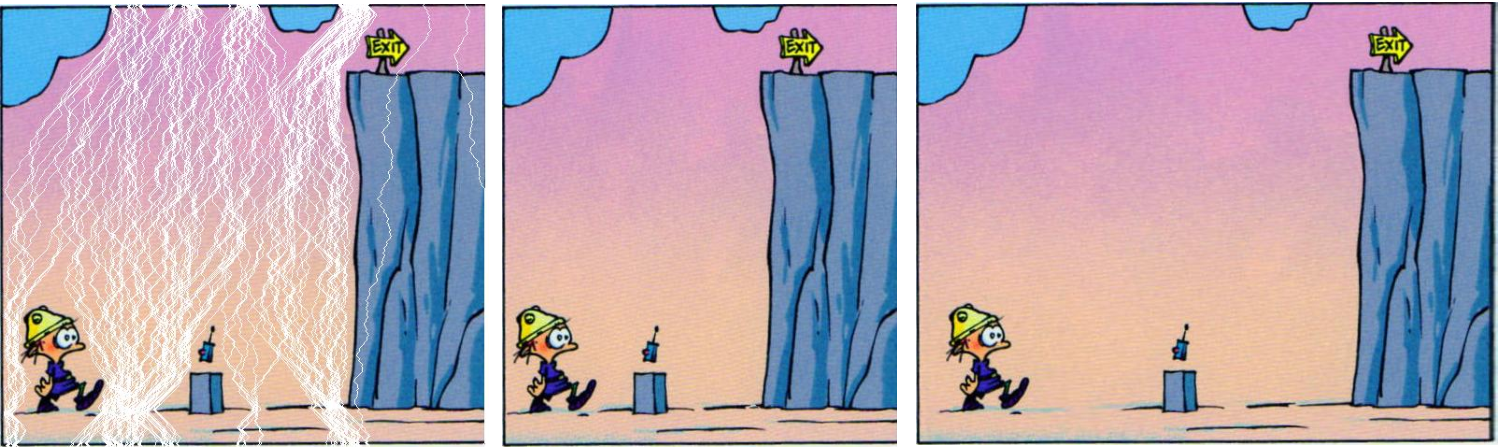
\includegraphics[width=14cm]{exemple-carving.pdf}}
\caption{\`A gauche, l'image de départ où les 100 coutures de coût
  minimal sont représentées en blanc. Au centre, la version réduite de
  l'image obtenue en supprimant ces 100 coutures. A droite, la version
  étendue obtenue en dupliquant ces
  coutures. \label{ref:exempleseamcarving}}
\end{figure}

\subsubsection{\'Elargissement d'une image}\label{sec:enlarge}

La même technique peut être utilisée pour augmenter artificiellement
la largeur d'une image. La procédure fonctionne de la manière suivante
(pour étendre l'image de $k$ pixels en largeur):
\begin{itemize}
\item On détermine exactement comme dans le cas de la réduction les
  $k$ coutures d'énergie minimale. Le résultat de cette opération
  devra être un marquage des pixels de l'image originale qui aurait du
  être supprimés si on avait effectué une réduction plutôt qu'un
  élargissement.
\item On parcourt l'image de gauche à droite et de haut en bas. Chaque
  pixel non marqué à l'étape précédente est recopié tel quel dans
  l'image finale. Chaque pixel marqué est recopié également mais on
  ajoute un nouveau pixel à sa droite dans l'image finale dont la
  valeur (pour chaque couleur) est obtenue en moyennant la valeur du
  pixel marqué et du pixel à sa droite dans l'image originale. Si le
  pixel marqué se trouve sur le bord droit de l'image, la valeur
  ajoutée est simplement la valeur du pixel marqué.
\end{itemize}

Cette procédure ne donne pas de bon résultats si le nombre de pixels à
ajouter est trop important par rapport à la taille initiale de
l'image. Il est préférable dans ce cas de répéter l'opération
d'élargissement plusieurs fois avec un nombre moindre de pixels. Soit
$k'$ un paramètre fixé arbitrairement à 20\% de la taille de l'image,
on procédera comme suit pour étendre la taille de l'image de $k$
pixels lorsque $k>k'$:
\begin{itemize}
\item On élargit l'image de $k'$ pixels en utilisant la procédure
  ci-dessus
\item On répète cette opération tant que l'image obtenue n'a pas
  atteint la taille cible
\end{itemize}

%% On considérera deux cas différents:
%% \begin{itemize}
%% \item Changement d'une seule dimension de l'image ($m\times n$ vers
%%   $m'\times m$ avec $m'<m$ ou $m\times n$ vers $m\times n'$ avec
%%   $n'<n$)
%% \item Changement des deux dimensions de l'image ($m\times n$ vers
%%   $m'\times n'$ avec $m'<m$ et $n'<n$).
%% \end{itemize}

%% \subsubsection{Une seule dimension}

%% Pour réduire la largeur de l'image de $m$ vers $m'$, on appliquera
%% $m'-m$ fois les opérations suivantes:
%% \begin{enumerate}
%% \item On calcule l'énergie des pixels l'image.
%% \item On recherche la couture verticale d'énergie minimale $S_x^*$.
%% \item On crée une nouvelle image en enlevant les pixels de la couture
%%   $S_x^*$ de l'image.
%% \end{enumerate}

%% La procédure est évidemment similaire dans le cas d'une réduction de
%% la hauteur de l'image (les coutures verticales étant bien entendu
%% remplacée par des coutures horizontales).

%% \subsubsection{Deux dimensions}

%% Pour réduire à la fois la résolution horizontale et la résolution
%% verticale, on alternera la suppression de coutures optimales
%% horizontales ($n'-n$ au total) et verticales ($m'-m$). L'ordre
%% d'application des coutures a évidemment un impact sur le résultat et
%% il est possible de

%\subsection{Extension d'une image}

%% \subsection{Recadrage dynamique}

%% Dans le cadre d'une mise en pratique de l'algorithme de recadrage, un
%% utilisateur souhaitera typiquement visualiser son image recadrée à
%% différentes hauteur et largeur afin d'évaluer le résultat et choisir
%% la taille idéale (voir par exemple le site \url{http://rsizr.com/}
%% pour un outil de ce type). Le travail à effectuer pour passer d'une
%% taille $m$ à une taille $m'<m$ consistant à passer par toutes les
%% tailles intermédiaires, il serait avantageux d'éviter de refaire
%% plusieurs fois des mêmes calculs afin de fournir une réponse rapide à
%% l'utilisateur. En plus de la fonction \texttt{SeamCarving} définie
%% précédemment, on vous demande d'implémenter une nouvelle version de
%% cette fonction appelée \texttt{SeamCarvingCached} prenant les mêmes
%% arguments que \texttt{SeamCarving} mais implémentant un système de
%% cache permettant de ne pas recalculer deux fois les mêmes choses
%% inutilement entre deux appels successifs à la fonction.

\subsection{Génération de la bande dessinée}\label{sec:packing}

Les différentes étapes pour générer la bande dessinée sur base d'une
liste de cases et d'une largeur de page seront les suivantes:
\begin{itemize}
\item Récupération des largeurs des cases et détermination de leurs
  positions optimales en fonction de la largeur cible.
\item Pour chaque rangée de la bande dessinée:
\begin{itemize}
\item Calcul de la réduction ou de l'élargissement à appliquer à
  chaque case. On répartira de manière équitable la réduction ou
  l'élargissement nécessaire sur chacune des cases de la rangée (aux
  arrondis près).
\item Application de la transformation (réduction ou expansion) à
  chaque case de la rangée et placement des cases sur l'image finale.
\end{itemize}
\end{itemize}

Pour donner un aspect visuel plus agréable, on ajoutera une bordure
blanche de taille fixée entre les cases et autour de l'image. La
largeur de ce bord devra être pris en compte notamment lors du calcul
du placement des cases. Les largeurs de cases soumises à l'algorithme
de répartition seront simplement augmentées de la largeur du bord et
la largeur de page sera diminuée de la largeur du bord (pour tenir
compte du bord à gauche).

\section{Directives d'implémentation}

On vous demande d'implémenter l'algorithme de mise en page intelligent
décrit ci-dessus. Vous devrez implémenter les fonctions suivantes
(voir le fichier 'ComicsPacking.h' pour les prototypes de ces
fonctions).

\paragraph{\texttt{BoxWrapping}.} Cette fonction calculera le placement optimal des cases. Elle prendra comme arguments le nombre de cases, un tableau reprennant la taille de chaque case et une largeur de page $W$. La sortie de cette fonction sera une table de taille $n$ reprenant pour chaque case la rangée à laquelle est doit être placée.

\paragraph{\texttt{ImageWidthReduction}.} Cette fonction implémentera la réduction d'une image par la technique décrite dans la section \ref{sec:reduc}. Elle prendra en argument une image (le format d'une image est décrit également dans le fichier 'ComicsPacking.h') et un nombre de pixels et elle renverra une nouvelle image obtenue en réduisant l'image initiale de $k$ pixels.

%% Note:
%% \begin{itemize}
%% \item La mise à jour de l'énergie peut se faire efficacement sans
%%   repasser sur toute l'image, en suivant la couture
%% \item Vous représenterez avantageusement la couture par une tableau de
%%   taille $m$ dont l'élément $i$ représentera la colonne correspondant
%%   à la couture.
%% \end{itemize}

\paragraph{\texttt{ImageWidthExpansion}.} Cette fonction implémentera l'élargissement d'image suivant la technique décrite dans la section \ref{sec:enlarge}. Elle prendra en argument une image et un nombre $k$ de pixels et renverra une nouvelle image élargie de $k$ pixels.

\paragraph{\texttt{ComicPacking}.} Cette fonction sera la fonction principale de votre programme. Elle prendra en argument un nombre de cases, un tableau d'images (les cases de la BD), une largeur de page et une épaisseur de bord. Elle fournira en sortie une nouvelle image contenant la planche complète générée selon la procédure décrite dans la section \ref{sec:packing}.

Pour vous aider dans vos tests, nous vous fournissons également deux
fichiers ``main'':
\begin{itemize}
\item mainSeamCarving.c: qui prend en argument sur la ligne de
  commande un nom de fichier image et un nombre de pixels (positif ou
  négatif) et renvoie dans un nouveau fichier l'image réduite (si le nombre
  de pixels est négatif) ou étendue (si le nombre de pixels est
  positif) à l'aide de vos fonctions \texttt{ImageWidthReduction} et
  \texttt{ImageWidthExpansion}.
\item mainComicPacking.c: qui prend en argument sur la ligne de
  commande une largeur d'image, un nombre de cases et une entête de
  nom de fichier et renvoie dans un fichier l'image de la bande
  dessinée générée à partir des cases.
\end{itemize}
Ces fichiers font appel aux fonctions de chargement et d'écriture d'images fournies dans les fichiers 'Image.h' et 'Image.c'.

%% \subsection{\texttt{SeamCarvingCached}}

%% Dans le cadre d'une mise en pratique de l'algorithme de recadrage, un
%% utilisateur souhaitera typiquement visualiser son image recadrée à
%% différentes hauteur et largeur afin d'évaluer le résultat et choisir
%% la taille idéale (voir par exemple le site \url{http://rsizr.com/}
%% pour un outil de ce type). Le travail à effectuer pour passer d'une
%% taille $m$ à une taille $m'<m$ consistant à passer par toutes les
%% tailles intermédiaires, il serait avantageux d'éviter de refaire
%% plusieurs fois des mêmes calculs afin de fournir une réponse rapide à
%% l'utilisateur. En plus de la fonction \texttt{SeamCarving} définie
%% précédemment, on vous demande d'implémenter une nouvelle version de
%% cette fonction appelée \texttt{SeamCarvingCached} prenant les mêmes
%% arguments que \texttt{SeamCarving} mais implémentant un système de
%% cache permettant de ne pas recalculer deux fois les mêmes choses
%% inutilement entre deux appels successifs à la fonction.

\section{Rapport}

%\renewcommand{\labelenumi}{(\alph{enumi})}

\begin{enumerate}
\item Pour chacun des deux algorithmes par programmation dynamique
  (répartition des cases et calcul de la couture d'énergie
  minimale):
\begin{enumerate}
\item Montrez qu'une approche par recherche exhaustive serait de
  complexité exponentielle (respectivement par rapport au nombre de
  cases et par rapport à la hauteur de l'image).
\item Donnez la formulation récursive complète de la fonction de coût
  (respectivement $c(n)$ et $C(i,j)$), en précisant bien les cas de base.
\item Représentez le graphe des appels récursifs pour un problème de
  petite taille.
\item Décrivez en pseudo-code un algorithme efficace de calcul des
  valeurs de cette fonction de coût (par l'approche ascendante ou
  descendante).
\item Donnez la complexité en temps et en espace de cet algorithme.
\end{enumerate}
\item Pour chacune des deux fonctions \texttt{ImageWidthReduction} et \texttt{ImageWidthExpansion}:
\begin{enumerate}
\item Décrivez vos choix d'implémentation.
\item Précisez leurs complexités en temps et en espace en fonction de
  la taille de l'image, $n\times m$, et du nombre $k$ de pixels à
  supprimer ou à enlever.
\end{enumerate}
\end{enumerate}

%\section*{Annexe: Liste des fichiers fournis et à rendre}
%A compléter.

\bibliography{p3bib}
\bibliographystyle{alpha}

\end{document}
